\titledquestion{Automatic differentiation}

Let
\[
    f(x,Q)=x^\top Qx-1,
    \qquad
    x=\begin{bmatrix}1\\2\end{bmatrix},
    \qquad
    Q=\begin{bmatrix}1&2\\3&4\end{bmatrix},
\]
where $Q$ is not assumed to be symmetric. We evaluate this function as
\[
    s=Qx, \qquad t=x^\top s, \qquad f=t-1.
\]
The corresponding expression graph and forward values are shown below. An
arrow points from each argument to the operation that uses it.

\begin{center}
    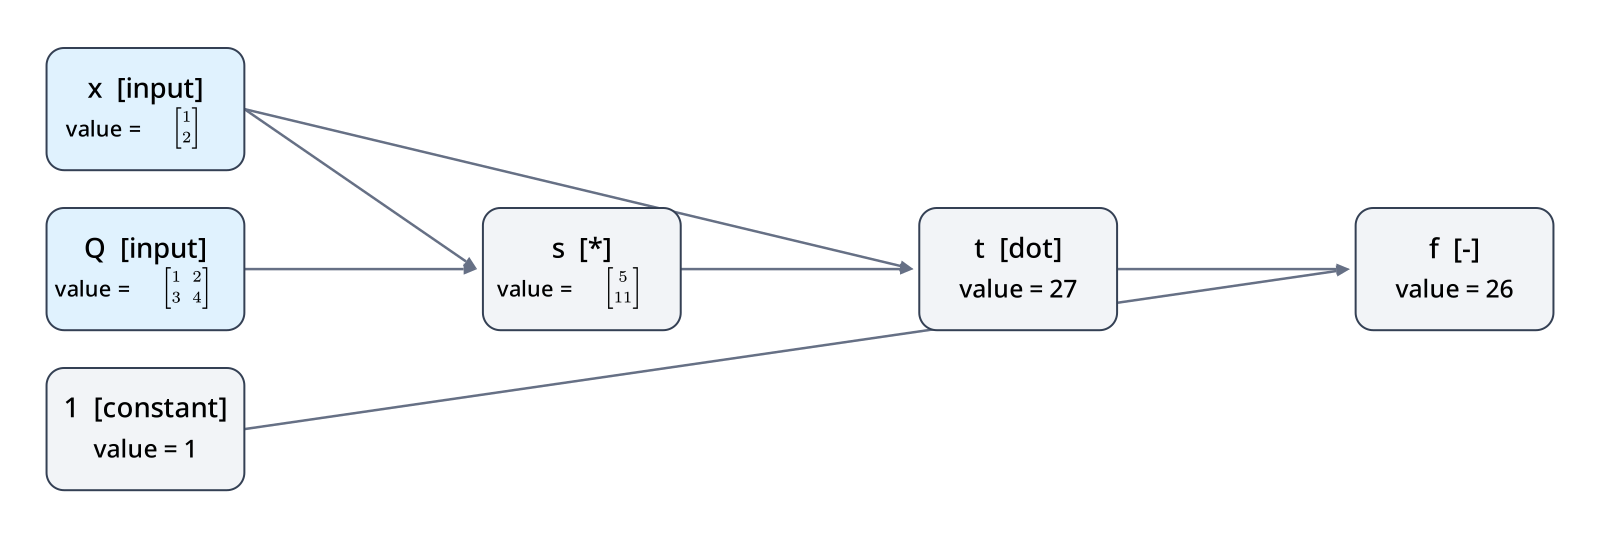
\includegraphics[width=0.9\linewidth]{ad_graph}
\end{center}

\begin{itemize}
    \item Starting with $\bar f=\partial f/\partial f=1$, perform the reverse
    pass. Give the order in which you process the operation nodes and show how
    the adjoint of $x$ accumulates its two contributions.

    \begin{solutionbox}{9cm}
        A valid reverse topological order is $f$, $t$, then $s$. From
        $f=t-1$, we obtain
        \[
            \bar t \mathrel{+}=\bar f=1.
        \]
        From $t=x^\top s$, we obtain
        \[
            \bar x \mathrel{+}=\bar t\,s
                =\begin{bmatrix}5\\11\end{bmatrix},
            \qquad
            \bar s \mathrel{+}=\bar t\,x
                =\begin{bmatrix}1\\2\end{bmatrix}.
        \]
        Finally, from $s=Qx$,
        \[
            \bar Q \mathrel{+}=\bar s x^\top
                =\begin{bmatrix}1&2\\2&4\end{bmatrix},
            \qquad
            \bar x \mathrel{+}=Q^\top\bar s
                =\begin{bmatrix}7\\10\end{bmatrix}.
        \]
        Hence the two contributions to $\bar x$ accumulate to
        \[
            \bar x=
            \begin{bmatrix}5\\11\end{bmatrix}
            +\begin{bmatrix}7\\10\end{bmatrix}
            =\begin{bmatrix}12\\21\end{bmatrix}.
        \]
    \end{solutionbox}

    \item Give $\nabla_x f$ and $\nabla_Q f$, first as formulas valid for
    arbitrary $x$ and $Q$, and then at the values above. Why does
    $\nabla_Q f$ have rank one whenever $x\ne0$?

    \begin{solutionbox}{8cm}
        The input adjoints give
        \[
            \nabla_x f=(Q+Q^\top)x,
            \qquad
            \nabla_Q f=xx^\top.
        \]
        At the specified values,
        \[
            \nabla_x f=\begin{bmatrix}12\\21\end{bmatrix},
            \qquad
            \nabla_Q f=\begin{bmatrix}1&2\\2&4\end{bmatrix}.
        \]
        For every vector $v$, $(xx^\top)v=x(x^\top v)$ belongs to
        $\operatorname{span}(x)$. Thus $xx^\top$ has rank at most one, and
        its rank is exactly one when $x\ne0$.
    \end{solutionbox}

    \item More generally, suppose that a scalar-valued function has many
    inputs. To compute its full gradient, which mode is usually preferable:
    forward or reverse? Briefly justify your answer.

    \begin{solutionbox}{4cm}
        Reverse mode is usually preferable. A single reverse pass computes
        the derivative of the scalar output with respect to every input,
        whereas forward mode generally requires one pass per input direction.
    \end{solutionbox}
\end{itemize}
